%%%%%%%%%%%%%%%%%%%%%%%%%%%%%%%%%%%%%%%%%
% a0poster Portrait Poster
% LaTeX Template
% Version 1.0 (22/06/13)
%
% The a0poster class was created by:
% Gerlinde Kettl and Matthias Weiser (tex@kettl.de)
% 
% This template has been downloaded from:
% http://www.LaTeXTemplates.com
%
% License:
% CC BY-NC-SA 3.0 (http://creativecommons.org/licenses/by-nc-sa/3.0/)
%
%%%%%%%%%%%%%%%%%%%%%%%%%%%%%%%%%%%%%%%%%

%----------------------------------------------------------------------------------------
%	PACKAGES AND OTHER DOCUMENT CONFIGURATIONS
%----------------------------------------------------------------------------------------

\documentclass[a0,portrait, final]{a0poster}

\usepackage{multicol} % This is so we can have multiple columns of text side-by-side
\columnsep=100pt % This is the amount of white space between the columns in the poster
\columnseprule=3pt % This is the thickness of the black line between the columns in the poster

\usepackage{titlesec}

\usepackage[svgnames]{xcolor} % Specify colors by their 'svgnames', for a full list of all colors available see here: http://www.latextemplates.com/svgnames-colors

\usepackage{times} % Use the times font
%\usepackage{palatino} % Uncomment to use the Palatino font

\usepackage{graphicx} % Required for including images
\graphicspath{{figures/}} % Location of the graphics files
\usepackage{booktabs} % Top and bottom rules for table
\usepackage{amsfonts, amsmath, amsthm, amssymb} % For math fonts, symbols and environments
\usepackage{wrapfig} % Allows wrapping text around tables and figures
\usepackage[utf8]{inputenc}
\usepackage{subcaption}
\usepackage[spanish, mexico]{babel}
\usepackage[utf8]{inputenc}
\usepackage{dblfloatfix}
% \usepackage{capt-of}%%To get the caption


\titlespacing\section{10pt}{12pt plus 4pt minus 1pt}{10pt plus 2pt minus 2pt}
% \setlength{\multicolsep}{6.0pt plus 2.0pt minus 1.5pt}% 50% of original values


\begin{document}

%----------------------------------------------------------------------------------------
%	POSTER HEADER 
%----------------------------------------------------------------------------------------

% The header is divided into two boxes:
% The first is 75% wide and houses the title, subtitle, names, university/organization and contact information
% The second is 25% wide and houses a logo for your university/organization or a photo of you
% The widths of these boxes can be easily edited to accommodate your content as you see fit


\begin{minipage}[bt]{0.6\linewidth}
\veryHuge \color{NavyBlue} \textbf{TapeYty} 
\color{Black}\\[1cm] % Title
\Huge\textit{Sistema para la gestión de rutas de recolección de residuos sólidos urbanos usando modelado SIG}\\[1cm] % Subtitle
%\Huge\textit{An Exploration of Complexity}\\[2cm] % Subtitle
\LARGE \textbf{Andrea Benítez, Francisco Quiñónez, María E. García-Díaz, Jorge Meza, Diego P. Pinto-Roa}\\[0.5cm]
% \huge Universidad Nacional de Asunci\'on - 
% \LARGE Facultad Politécnica\\[0.4cm] 
\LARGE Universidad Nacional de Asunci\'on - 
\Large Facultad Politécnica\\[0.4cm] 
% University/organization
\large \texttt{\{abenitez, fquinonez, mgarcia, jmeza, dpinto\}@pol.una.py}
\end{minipage}
%
\begin{minipage}[bt]{0.4\linewidth}
\centerline{
\raisebox{-0.5\height}{
\includegraphics[scale=0.5]{./figures/logo.pdf}}
\raisebox{-0.5\height}{
\includegraphics[scale=1]{./figures/tapeYtyLogo.png}}}
\end{minipage}

\vspace{1cm} % A bit of extra whitespace between the header and poster content

%----------------------------------------------------------------------------------------

\begin{multicols}{2} % This is how many columns your poster will be broken into, a portrait poster is generally split into 2 columns



%----------------------------------------------------------------------------------------
%	INTRODUCTION
%----------------------------------------------------------------------------------------

%\color{SaddleBrown} % SaddleBrown color for the introduction

\section*{Introducci\'on}

El impacto ambiental que provocan los residuos sólidos municipales ha sido objeto de atención especial en las últimas décadas. La eliminación de los residuos sólidos urbanos es una preocupación creciente en todo el mundo, sin importar el tamaño ni las características socio-económicas de una ciudad \cite{Karadimas2007OptimalAlgorithm}. 
% Muchas ciudades se han visto obligadas a evaluar su programa de gestión de residuos sólidos y examinar su relación costo-efectividad en términos de recolección, transporte, tratamiento y eliminación \cite{Karadimas2007OptimalAlgorithm}.

En la Gestión de Residuos Sólidos se estima que de la cantidad total de dinero destinado para su recogida, transporte y eliminación, aproximadamente el 60-80\% se gasta en la fase de Recolección de Residuos Sólidos \cite{Tavares2009OptimisationModelling}. 
El área de estudio es Asunción, capital y ciudad más poblada de la República del Paraguay. La Dirección de Servicios Urbanos es la responsable de la recolección de residuos sólidos urbanos y divide la ciudad en 134 zonas para realizar la labor. Los recorridos en las zonas de trabajo son realizados en base a la experiencia e intuición de los conductores.

% En este trabajo se propone el desarrollo de una herramienta sobre una arquitectura modular e interoperable, que optimice el camino a seguir por los vehículos de recolección de basura domiciliaria de Asunción mediante técnicas de programación matemáticas y GIS.

% y consecuentemente, genere beneficios principalmente en el aspecto económico con la disminución de la distancia recorrida y en consecuencia el consumo de combustible; y ambiental con la disminución de la emisión de gases que dejan a su paso los camiones debido al menor tiempo de actividad \cite{Vu2018ParameterModel}


%----------------------------------------------------------------------------------------
%	OBJECTIVES
%----------------------------------------------------------------------------------------

\section*{Objetivo general}
El objetivo general de este trabajo de investigación es el de proponer una solución que optimice el recorrido de los vehículos de recolección de basura domiciliaria de la Dirección Servicios Urbanos (DSU) de la Municipalidad de Asunción.

\section*{Objetivos específicos}
\begin{enumerate}
    \item \textbf{Revisar} los enfoques de optimización de recolección de residuos sólidos.
    \item \textbf{Identificar} los factores que influyen en la recolección domiciliaria de la DSU.
    \item \textbf{Aplicar un enfoque} de optimización que mejor se ajuste a las reglas de negocio del caso de estudio.
    \item \textbf{Proponer y desarrollar una aplicación GIS} que permita configurar los parámetros de entrada del problema y despliegue la ruta óptima para cada zona de recolección.
    \item \textbf{Comparar} resultados de la aplicación desarrollada con los recorridos que actualmente son realizados, y de esta manera validar los resultados obtenidos.
\end{enumerate}

%----------------------------------------------------------------------------------------
%	MATERIALS AND METHODS
%----------------------------------------------------------------------------------------


\section*{Propuesta de solución}

En la actualidad, la DSU no cuenta con un \textit{software} que apoye a la toma de decisiones en lo que respecta a la gestión de residuos sólidos urbanos, más específicamente en el área de recolección. Se propone la implementación de una herramienta GIS que contribuya con la elección de mejores caminos a seguir por los vehículos recolectores en sus zonas de trabajo, y de esta manera generar mayores beneficios en cuanto a tiempo y distancia, además de garantizar que el servicio sea brindado a todos los contribuyentes.
% La herramienta APHOPe ha sido diseñada e implementada para que los médicos puedan generar los protocolos que utilizan para el tratamiento del paciente e introducir los datos de los mismos durante la realización de una consulta ambulatoria o una internación, de forma intuitiva y ágil, permitiendo además que esos datos queden almacenados en la base de datos de forma automática.  Además, se incluyen datos estadísticos que obtiene información del protocolo aplicado a cada paciente de manera que los médicos puedan tener información útil para la toma de decisiones y para el análisis de efectividad del protocolo. Los módulos componentes del APHOPe se observan en la Figura \ref{fig:componentes}.

% \begin{center}
%     \includegraphics[width=27cm, height=15cm]{./figures/componentes.jpg}
%     \captionof{figure}{ Componentes de APHOPe}
%     \label{fig:componentes}
% \end{center}
% \begingroup
%     \centering
%     \includegraphics[scale=1.5]{./figures/componentes.jpg}
%     \captionof{figure}{This is the caption}\label{fig:a}
% \endgroup

\section*{Metodología}
En la Figura \ref{fig:metodologia} se muestra la metodología seguida en este trabajo: la recolección de datos, el modelado matemático, la implementación de la herramienta \textit{TapeYty}, el despliegue de la ruta óptima y por último el análisis de los resultados.
% La Ingeniería de \textit{Software} es el proceso formal de desarrollo de \textit{software} en el que las necesidades del usuario se traducen en requerimientos, estos se transforman en diseño que se implementa en código que se prueba, documenta y se certifica para su uso operativo\cite{bauer}. La ingeniería de \textit{software} es una tecnología con varias capas, en la Figura \ref{fig:metodologia} se detallan las actividades realizadas en cada una de ellas.

\begin{center}
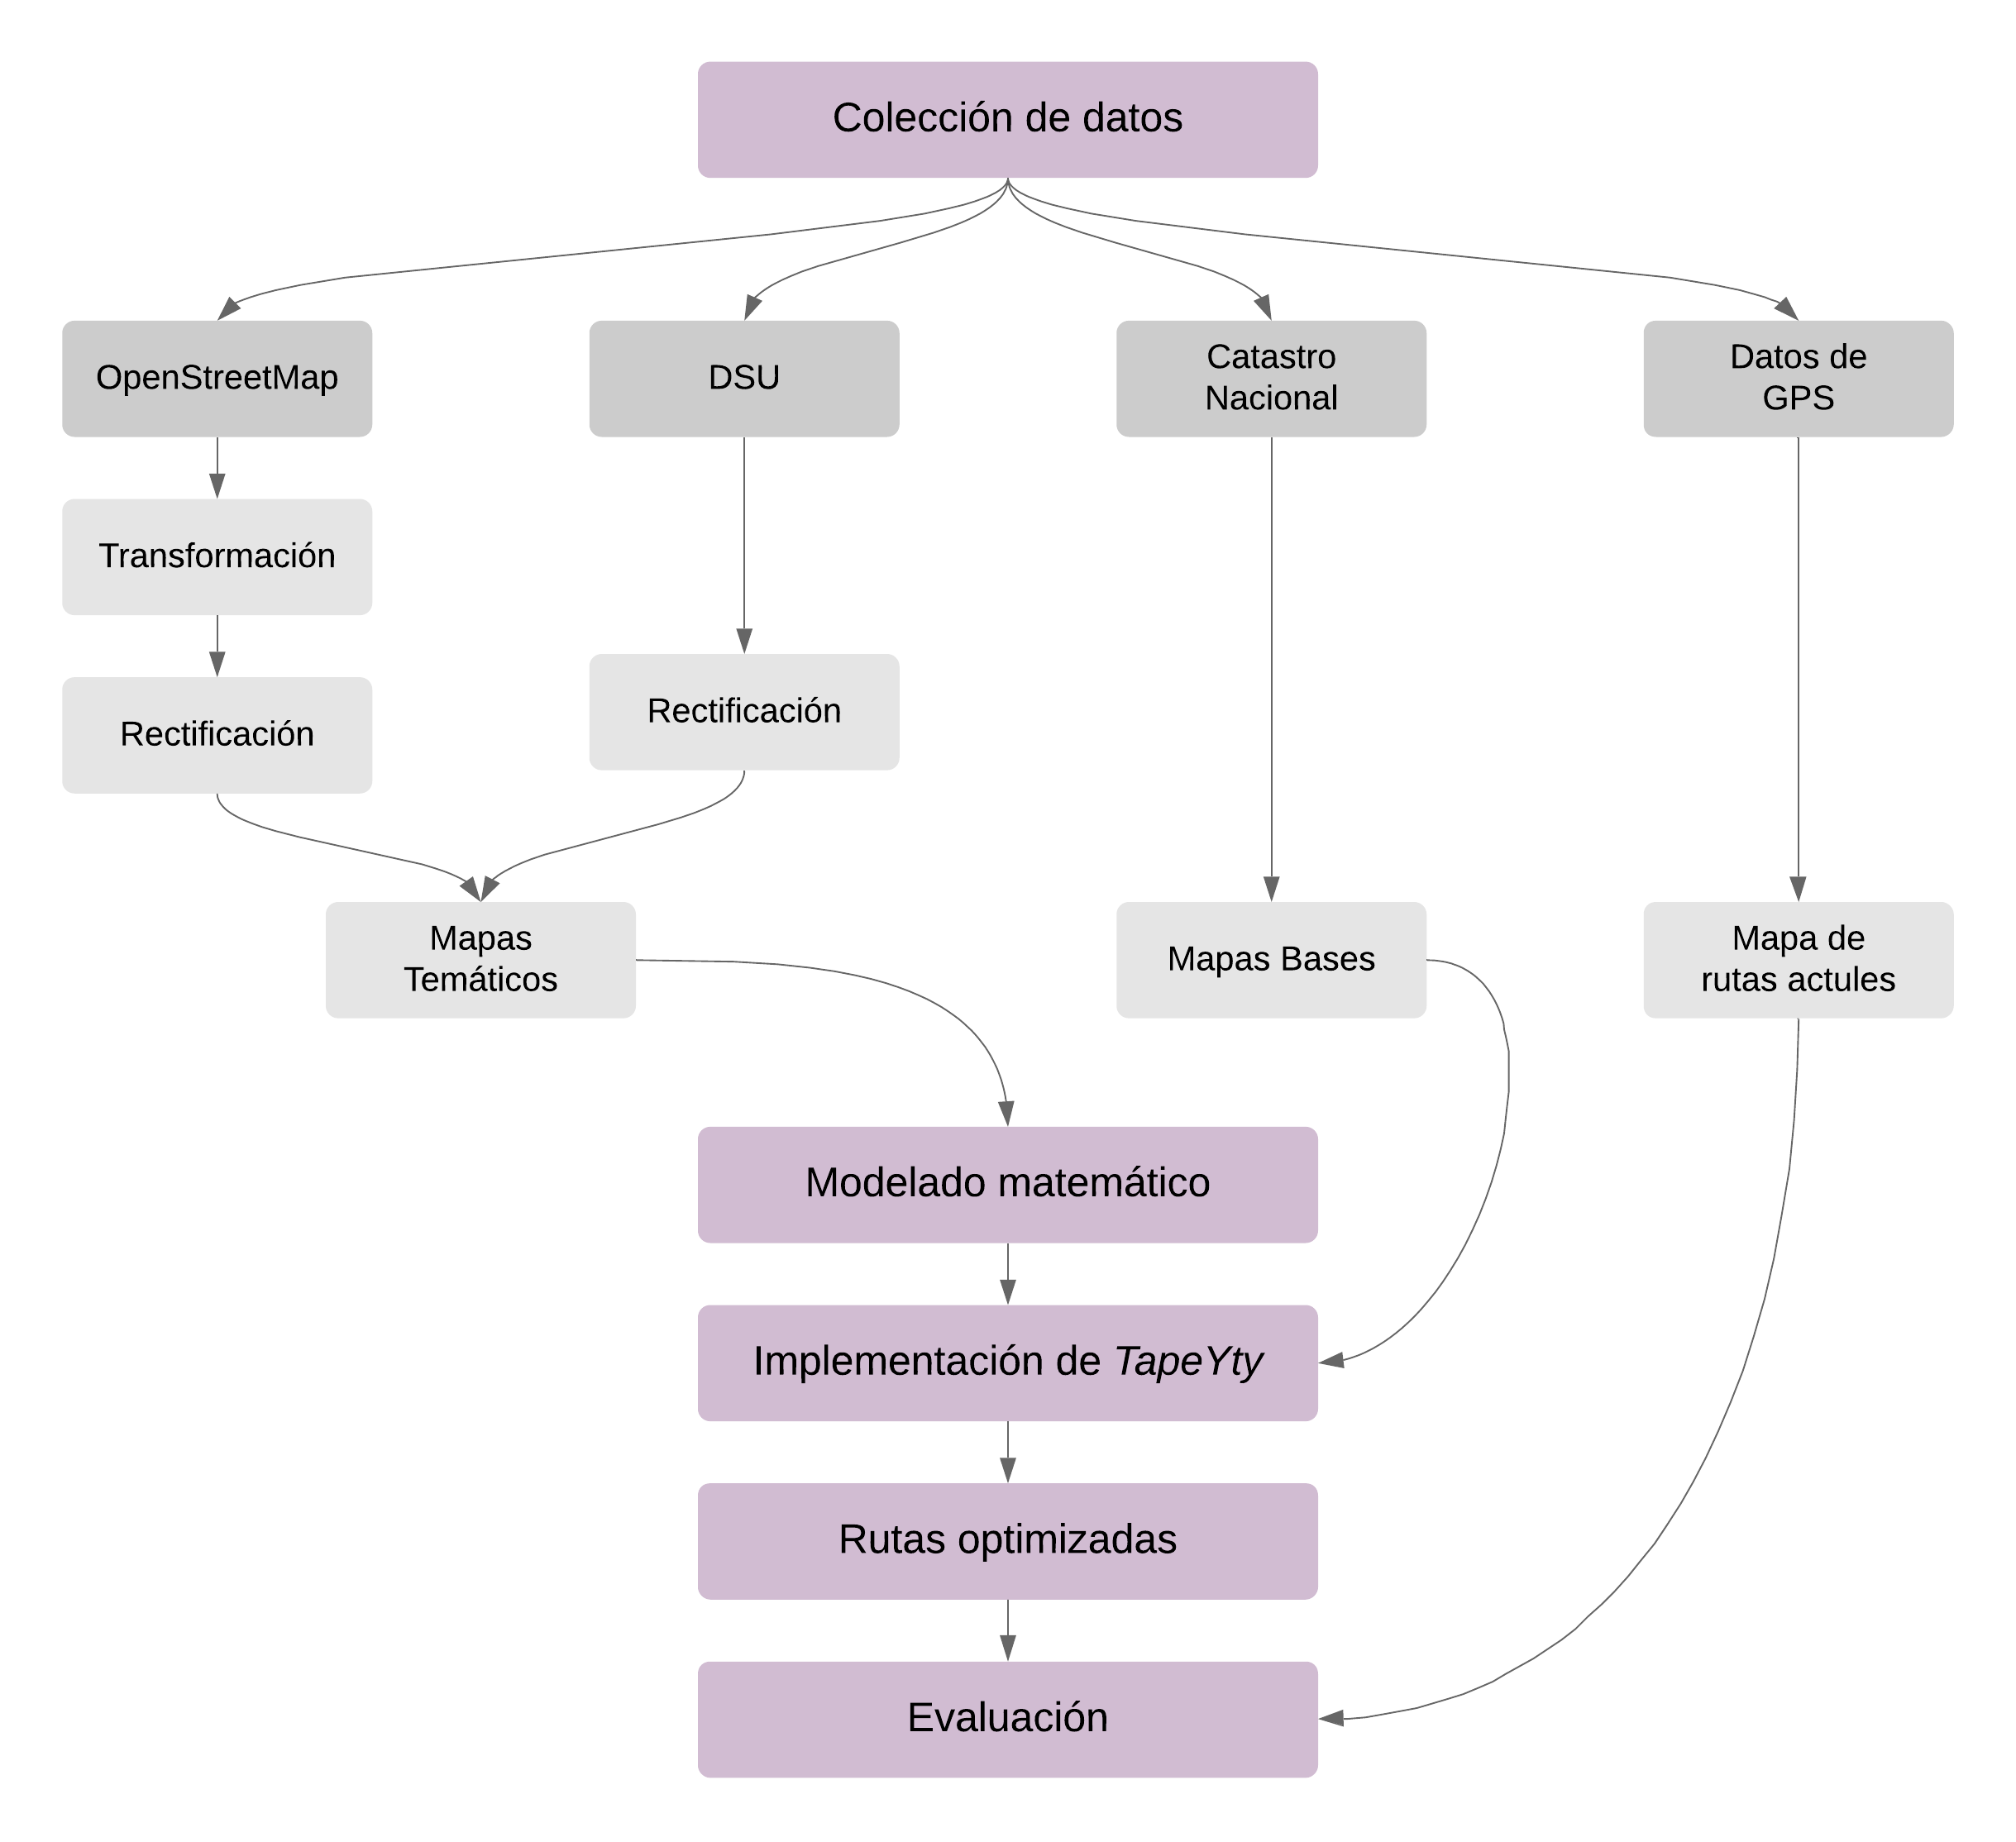
\includegraphics[scale=1.5]{./figures/DiagramaDeMetodologia.png}
    \captionof{figure}{Vista general de los procesos de la metodología aplicada.}
    \label{fig:metodologia}
\end{center}

% \begin{center}
% 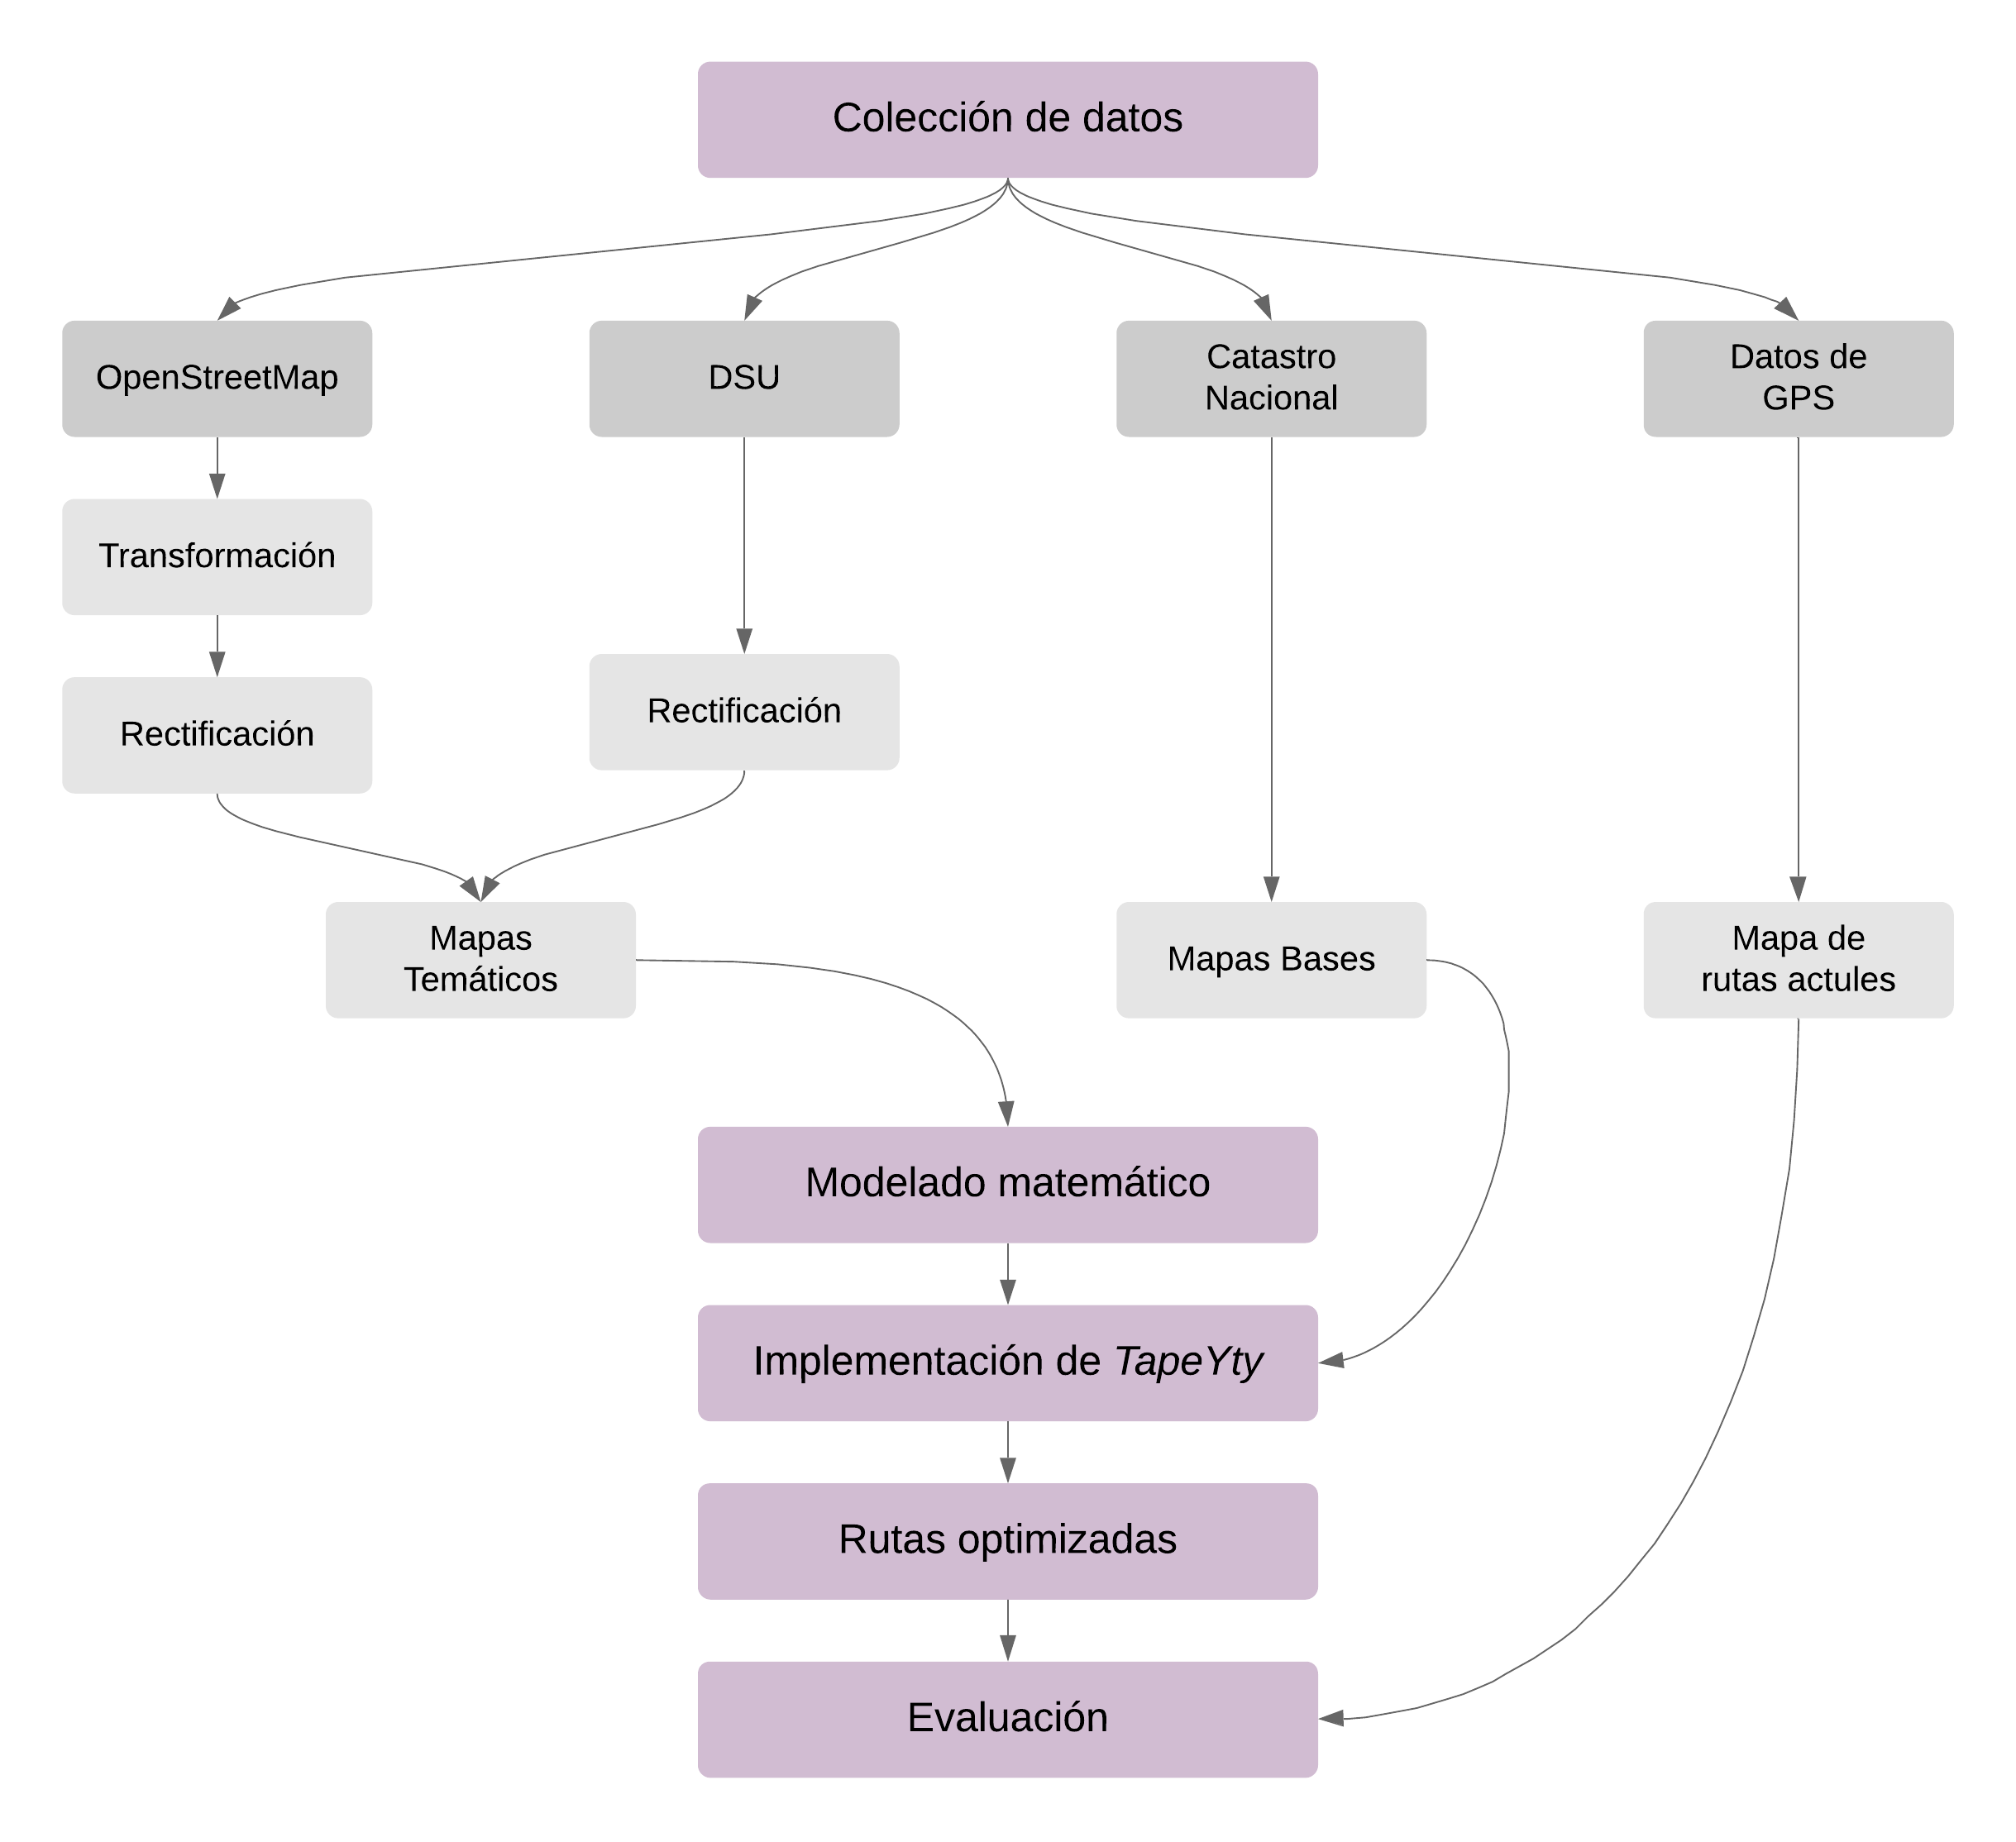
\includegraphics[scale=1.5]{./figures/DiagramaDeMetodologia.png}
%     \captionof{figure}{Etapas de la Ingeniería de \textit{Software} \cite{sommerville}}
%     \label{fig:metodologia}
% \end{center}

Para el desarrollo de la aplicación se aplicó una adaptación de la metodología ágil Scrum, ya que a lo largo del trabajo se superpusieron los roles de Equipo de desarrollo, \textit{Product Owner} y Scrum Master.
% Para realizar cada una de las etapas de la Ingeniería de \textit{Software} utilizamos aspectos del modelo en cascada y el modelo \textit{Scrum}, el trabajo no es puramente ágil. 
\section*{Resultados y discusiones}

En la Figura \ref{fig:distancias} se observa una comparación entre la distancia del recorrido realizado por los conductores en base a su experiencia y los caminos generados por TapeYty. Se realizaron dos escenarios de prueba con TapeYty. Uno donde se simuló el camino recorrido por el conductor, es decir, si el conductor no pasó por un tramo de calle, entonces el mismo fue configurado como opcional en la aplicación. Los resultados de este escenario se muestran en la tercera columna con un promedio de mejora de 19,28\% sobre las 6 zonas tomadas en cuenta.
El segundo escenario consistió en configurar todos los tramos de calles de la zona como requeridos. Se puede observar que el promedio de mejora disminuye a un 12,48\%, ya que no se configuro ningún tramo como opcional.

Estos resultados son validados por la literatura \cite{Braier2017AnArgentina, Vu2018ParameterModel}, donde al reducir la distancia recorrida se generan beneficios tanto en el aspecto económico debido al menor consumo de combustible como en el ambiental con la disminución de la emisión de gases que dejan a su paso los camiones debido al menor tiempo de actividad.

\begin{center}
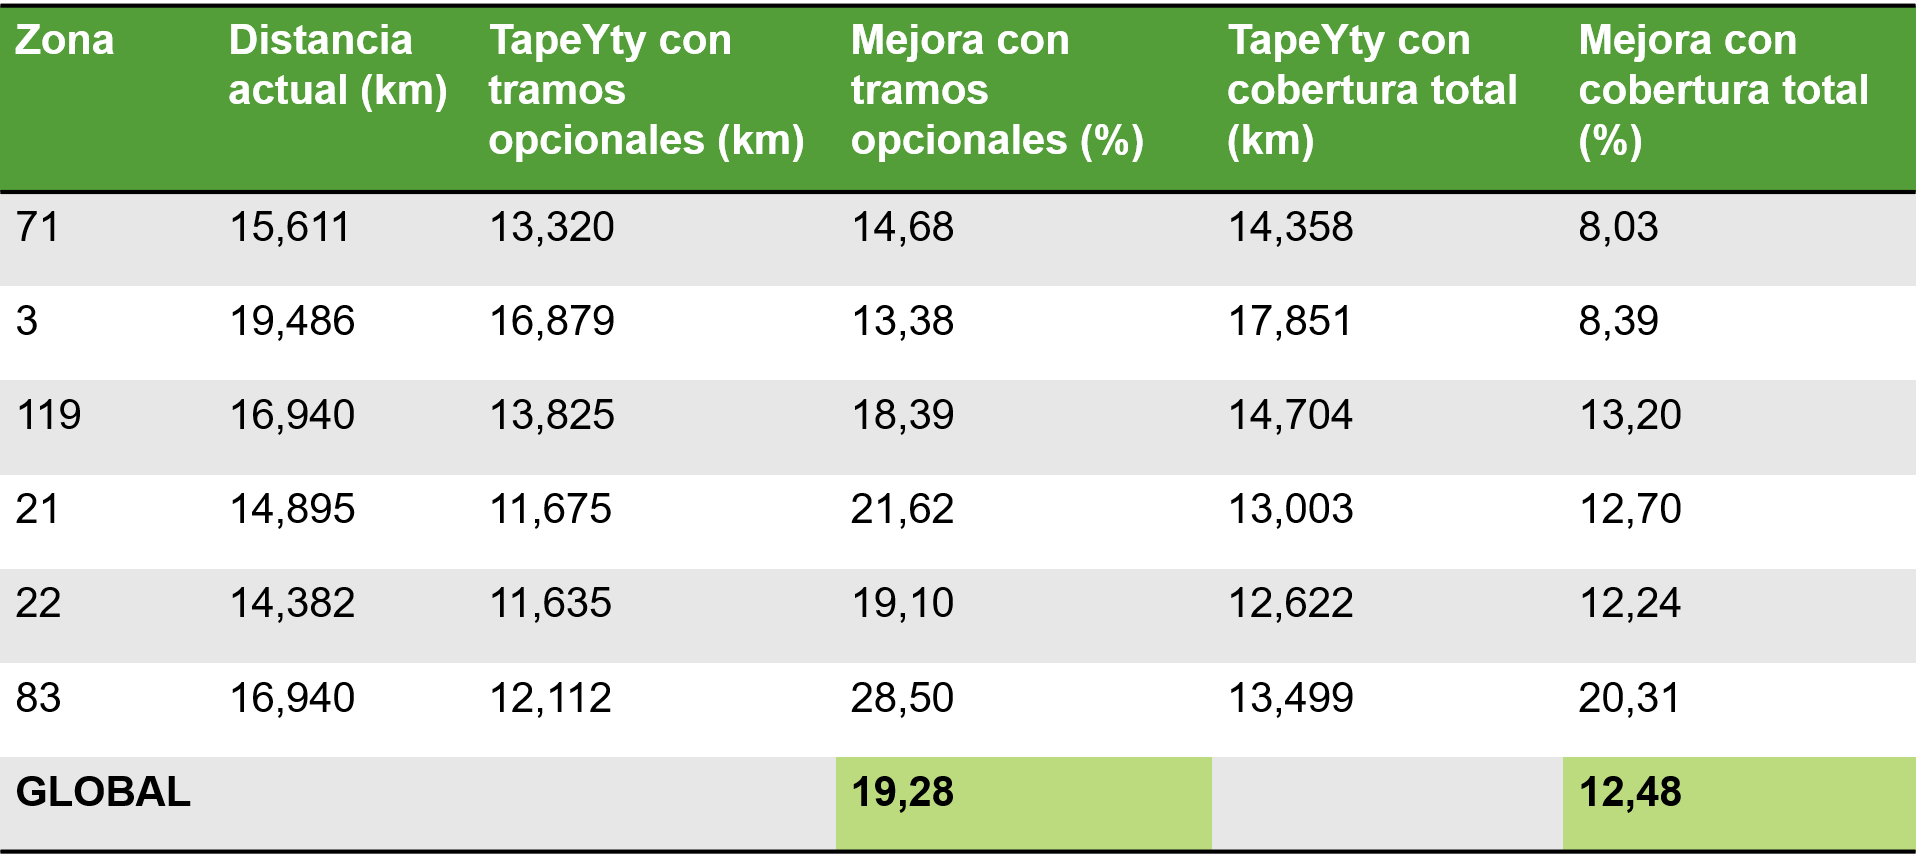
\includegraphics[width=0.45\textwidth]{./figures/resultadoComparacionDistancias.png}
    \captionof{figure}{Resultados de comparación de distancias.}
    \label{fig:distancias}
\end{center}

% \begin{table}[h]
% \centering
% \caption{Resultados de comparación de distancias}
% \label{table:distancias}
% \begin{tabular}{|l|l|l|l|l|l|}
% \hline
% Zona & Distancia actual (km) & \begin{tabular}[c]{@{}l@{}}TapeYty con tramos \\ opcionales (km)\end{tabular} & \begin{tabular}[c]{@{}l@{}}Mejora con tramos\\ opcionales (\%)\end{tabular} & \begin{tabular}[c]{@{}l@{}}TapeYty con cobertura\\ total (km)\end{tabular} & \begin{tabular}[c]{@{}l@{}}Mejora con cobertura\\ toal (\%)\end{tabular} \\ \hline
% 71 & 15.611 & 13.320 & 14.68 & 14.358 & 8.03 \\ \hline
% 3 & 19.486 & 16.879 & 13.38 & 17.851 & 8.39 \\ \hline
% 119 & 16.940 & 13.825 & 18.39 & 14.704 & 13.20 \\ \hline
% 21 & 14.895 & 11.675 & 21.62 & 13.003 & 12.7 \\ \hline
% 22 & 14.382 & 11.635 & 19.10 & 12.622 & 12.24 \\ \hline
% 83 & 16.940 & 12.112 & 28.50 & 13.499 & 20.31 \\ \hline
% Global &  &  & \textbf{19.28} &  & \textbf{12.18} \\ \hline
% \end{tabular}
% \end{table}

\begin{center}
    \centerline{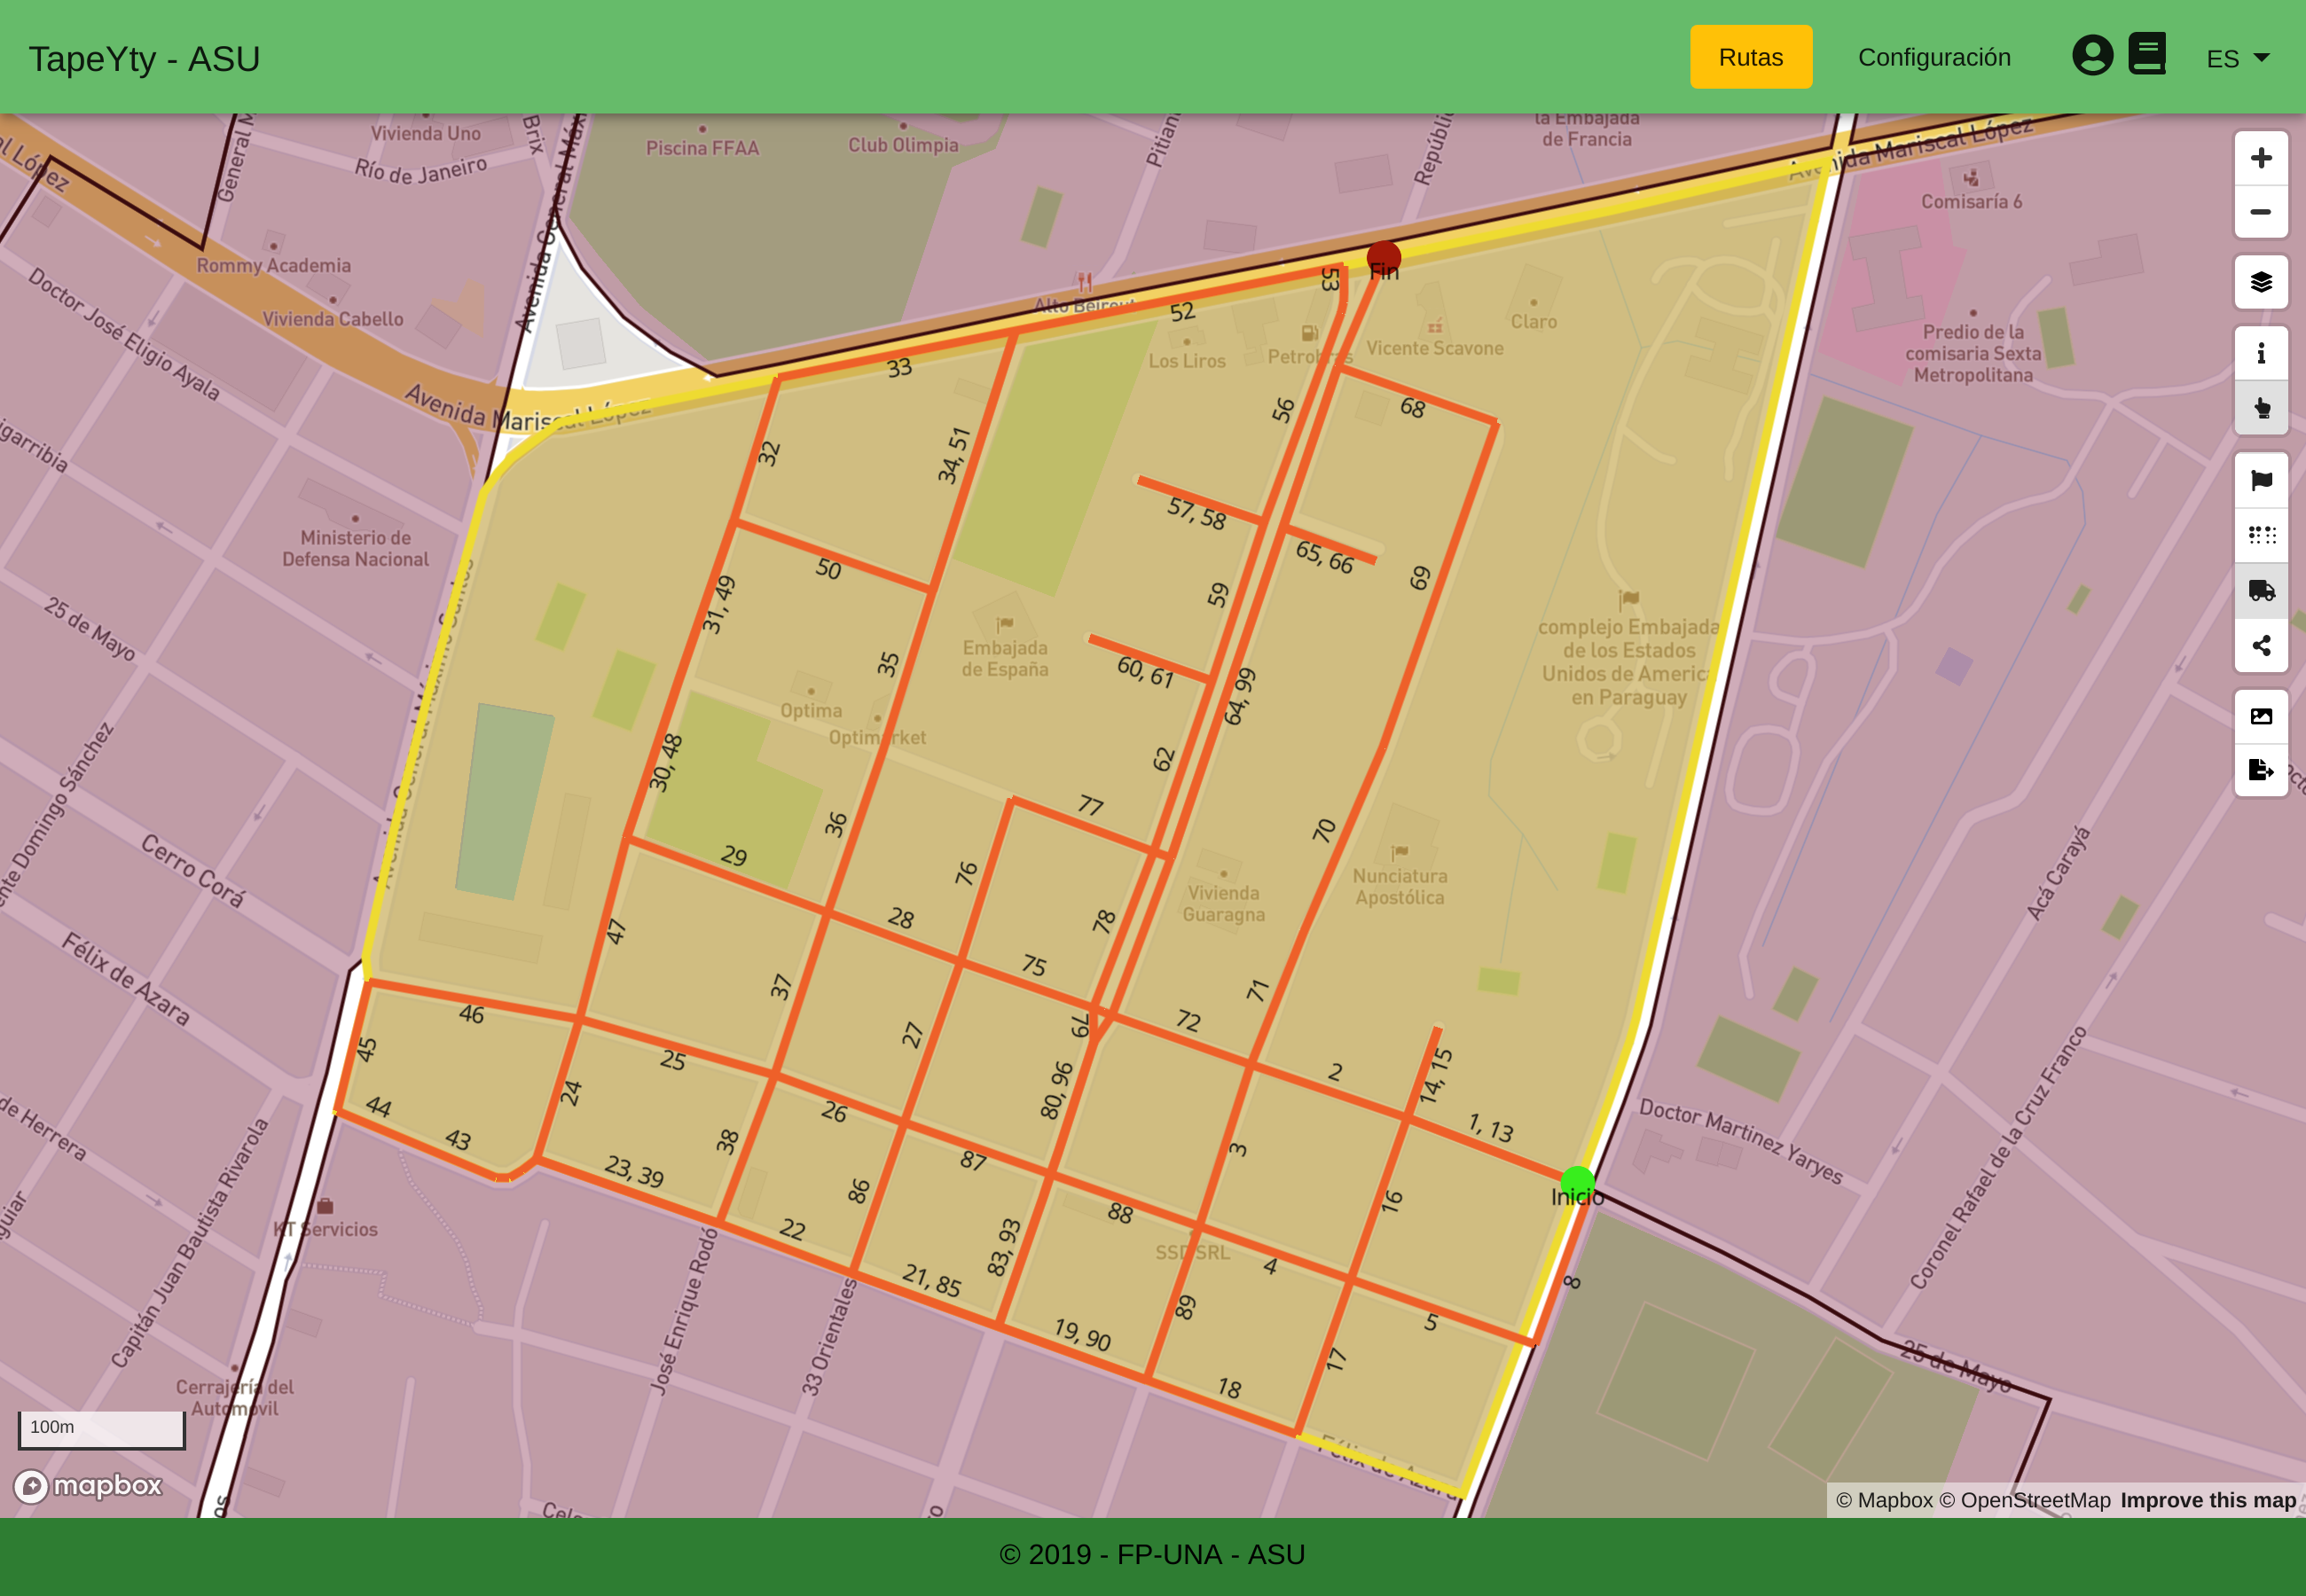
\includegraphics[width=0.45\textwidth]{./figures/recorrido.png}}
    \captionof{figure}{Despliegue de ruta generada por TapeYty en una zona de trabajo}
\end{center}
%----------------------------------------------------------------------------------------
%	CONCLUSIONS
%----------------------------------------------------------------------------------------

%\color{SaddleBrown} % SaddleBrown color for the conclusions to make them stand out

\section*{Conclusi\'on}
% En ciudades en vías de desarrollo, como Asunción, el trayecto seguido por el conductor del vehículo de recolección de basura se basa en su propia intuición y experiencia debido a la falta de herramientas que ayuden a la toma de decisiones. 

TapeYty utiliza los principales enfoques encontrados en la literatura en lo que respecta a la recolección de residuos sólidos: técnicas de programación matemática y GIS. De acuerdo a los datos que se pudieron recabar, los factores que se tienen en cuenta para la generación de un nuevo recorrido son: las reglas de circulación de la red de rutas, estados de calles y definición de las zonas de recolección. La metodología de trabajo en la DSU se ajusta al problema del cartero rural abierto, y se optó por implementar la solución propuesta por \cite{Braier2017AnArgentina}.
% En este trabajo se analizaron varias propuestas de solución del estado del arte con respecto a la recolección de residuos sólidos domiciliarios. La metodología de trabajo en la DSU se ajusta al problema del cartero rural abierto, por lo que se utiliza la solución propuesta por \citet{Braier2017AnArgentina}

Se diseñó y desarrolló TapeYty, un sistema hecho a medida para la DSU que fue resultado del relevamiento llevado a cabo en dicha institución. Es el primer sistema presentado a la DSU en lo que respecta a la gestión de rutas en las zona de trabajos. Se evidencia que aunque se mantenga el procedimiento de recolección, la distancia del recorrido es mejorada, además se garantiza que todos los segmentos serán cubiertos por la recolección.

%\color{DarkSlateGray} % Set the color back to DarkSlateGray for the rest of the content

%----------------------------------------------------------------------------------------
%	FORTHCOMING RESEARCH
%----------------------------------------------------------------------------------------
\section*{Aportes}
El sistema TapeYty; El Manual de usuario y guía técnica; El artículo científico.
% \begin{enumerate}
% \item El sistema TapeYty.
% \item El Manual de usuario y técnico.
% \item El artículo científico.
% \end{enumerate}

\section*{Trabajos futuros}

Como líneas de trabajos futuros, se propone considerar el relieve del camino como un factor en la generación de ruta \cite{Sulemana2018OptimalMethods}, y compararla con el modelo implementado en este trabajo, teniendo en cuenta que el centro de la ciudad de Asunción y alrededores está levantada sobre 7 (siete) colinas; Crear una mesa de trabajo con la DSU para obtener los datos relacionados a los kilogramos de residuos domiciliarios recolectados diariamente y estudiar la conveniencia de reorganizar las zonas y turnos de trabajo; Aprovechar la escalabilidad de la arquitectura implementada para agregar la optimización de las rutas para recolección de los residuos de grandes generadores; Integrar al sistema el monitoreo del recorrido y permitir al conductor regenerar una nueva ruta desde el último punto registrado, teniendo en cuenta los tramos de calles ya visitados.

 %----------------------------------------------------------------------------------------
%	REFERENCES
%----------------------------------------------------------------------------------------

% \nocite{*}
% Print all references regardless of whether they were cited in the poster or not
\bibliographystyle{IEEEtran} % Plain referencing style
\bibliography{references} % Use the example bibliography file sample.bib

%----------------------------------------------------------------------------------------
%	ACKNOWLEDGEMENTS
%----------------------------------------------------------------------------------------

% \section*{Acknowledgements}

% Etiam fermentum, arcu ut gravida fringilla, dolor arcu laoreet justo, ut imperdiet urna arcu a arcu. Donec nec ante a dui tempus consectetur. Cras nisi turpis, dapibus sit amet mattis sed, laoreet.

%----------------------------------------------------------------------------------------

\end{multicols}
\end{document}